\par \Note Оценки см. в прошлом билете (54)

\par \textbf{Теорема (Борсука–Улама–Люстерника–Шнирельмана):} $S^{n-1} \subset \mathbb{R}^n$ - сфера в $n$-мерном пространстве, $S^{n-1}=A_1 \cup \ldots \cup A_n$, $\forall i \: A_i$ - замкнуто или открыто. Тогда $\exists i, \: \exists \overline{x} \in A_i: \: -\overline{x} \in A_i$.

\par \textbf{Теорема (Ловас):} $\chi(KG_{n,k})\geq n-2k+2$
\par \Proof Пусть $\chi(G) < n-2k+1=d$. Обозначим цвета как $\chi_1, \ldots, \chi_d$, обозначим $\chi(K)$ - цвет вершины $K$. Тогда $$\forall K_i, K_j \subset \{1, \ldots, n\}: \: |K_i|=|K_j|=k, \: K_i \cap K_j=\varnothing \hookrightarrow \chi(K_i) \neq \chi(K_j)$$

\par Рассмотрим $S^d \subset \mathbb{R}^{d+1}$. Выберем на $S_d$ точки $\overline{x_1}, \ldots, \overline{x_n}$ так, чтобы на каждом экваторе было $\leq d$ точек (экватор - любое центральное сечение сферы гиперплоскостью). Это можно сделать, просто последовательно выставляя точки не на те экваторы, которые уже заняты. Перепишем условие кнезеровского графа для наших точек $$\forall K_i, K_j \subset \{\overline{x_1}, \ldots, \overline{x_n}\}: \: |K_i|=|K_j|=k, \: K_i \cap K_j=\varnothing \hookrightarrow \chi(K_i) \neq \chi(K_j)$$

\par Рассмотрим произвольную точку $\overline{x}$. Обощначим за $H(\overline{x})$ верхнюю открытую полусферу с эпицентром $\overline{x}$ (см. картинку ниже)
\\
\begin{center}
    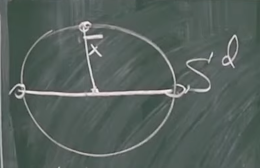
\includegraphics[scale=0.8]{images/dima_hemisphere.png}
\end{center}
\par Введем множества $A_i=\{\overline{x} \in S^d:$ в $H(\overline{x})$ есть хотя бы одна вершина $KG_{n,k}$ цвета $\chi_i\}, \: i=1,\ldots, d$. Заметим, что не все точки на сфере попали в какое-то $A_i$ - есть точки, в полусферах которых не лежит полностью ни одна из вершин кнезеровского графа (там мало точек). Введем $A_{d+1}=\{\overline{x}\in S^d: \: |H(\overline{x})\cap\{\overline{x_1}, \ldots, \overline{x_n}\}|\leq k-1\}$.

\par Очевидно, что множества $A_i$ при $i \leq d$ открыты (маленьким движением полусферы точки не пропадут из нее и не появятся в ней), а $A_{d+1}$ - замкнуто, как дополнение открытых. Тогда по теореме Борсука-Улама $\exists i: \: \exists \overline{x} \in A_i: \: -\overline{x} \in A_i$.

\newpage{}
\par Предположим, что $i\leq d$. Тогда в каждой из полусфер (см. картинку ниже) есть вершина кнезеровского графа цвета $\chi_i$. Они не пересекаются, так как лежат в непересекающихся полусферах, но они одного цвета - противоречие (помним, что в кнезеровском графе между вершинами есть ребро $\Leftrightarrow$ множества, соответствующие вершинам, не пересекаются). 
\\
\begin{center}
    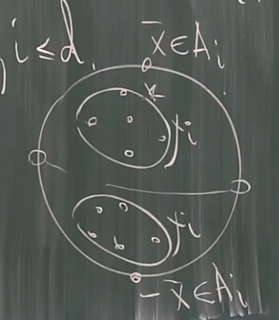
\includegraphics[scale=0.5]{images/dima_d.png}
\end{center}

\par Тогда $i=d+1$. Значит в обеих полусферах $\leq k-1$ точка (см. картинку ниже). Тогда на экваторе между ними $\geq n - 2(k-1)=n-2k+2>d$ точек - противоречие с расстановкой точек.
\\
\begin{center}
    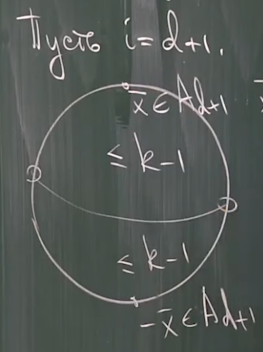
\includegraphics[scale=0.5]{images/dima_d+1.png}
\end{center}

\par Откуда следует, что $\chi(G) \geq n-2k+2$ и теорема доказана \EndProof